\documentclass[../main.tex]{subfiles}
\graphicspath{{\subfix{../images/}}}
\begin{document}


\section{Přímé metody pro řešení soustav lineárních algebraických rovnic}
Řešíme $\mathbb{A}x = b$, kde \matA je SPD matice.

Obecně: Řešení $\mathbb{A}x = b$ GEM $\Leftrightarrow$ přenásobení rozšířené matice soustavy maticemi 
elementárních úprav. 
\begin{equation*}
    \mathbb{L}_{n-1}\dots\mathbb{L}_{2}\mathbb{L}_{1}\mathbb{A} = \tilde{\mathbb{L}}\mathbb{A} = \mathbb{U}
\end{equation*}
$\mathbb{U}$ je matice v horním trojúhelníkovém tvaru, $\mathbb{L}$ je v dolním trojúhelníkovém tvaru.
\begin{equation*}
    \tilde{\mathbb{L}}\mathbb{A}=\mathbb{U} \Leftrightarrow \mathbb{A} = \tilde{\mathbb{L}}^{-1}\mathbb{U}
\end{equation*}

GEM je ekvivalentní konstrukci LU rozkladu matice \matA .

Algoritmus:
\begin{enumerate}
    \item Kostrukce $\mathbb{L}, \mathbb{U}$ tak, že $\mathbb{A} = \mathbb{L} y$, $O(n^3)$
    \item $\mathbb{L} y = b$, $O(n^2)$ - řeší zpětný chod
    \item $\mathbb{U} x = y$, $O(n^2)$ - řeší zpětný chod
\end{enumerate}


LU rozklad existuje $\Leftrightarrow$ \matA je silně negativní, pokud není je třeba přehazovat
řádky a sloupce matice \matA

SPD matice je silně negativní $\implies$ přehazovat řádky a sloupce není třeba.




Pro \matA SPD, $\mathbb{U} = \mathbb{L}^T$\\
$\mathbb{A} = \mathbb{L}\mathbb{L}^T$, kde $\mathbb{L}$ je v dolním trojúhelníkovém tvaru provedeme Choleského rozklad\\
$\mathbb{A} = \mathbb{L}\mathbb{D}\mathbb{L}^T$ - bezodmocninová metoda 





\subsection{Odvození Choleského rozkladu}

\begin{center}
    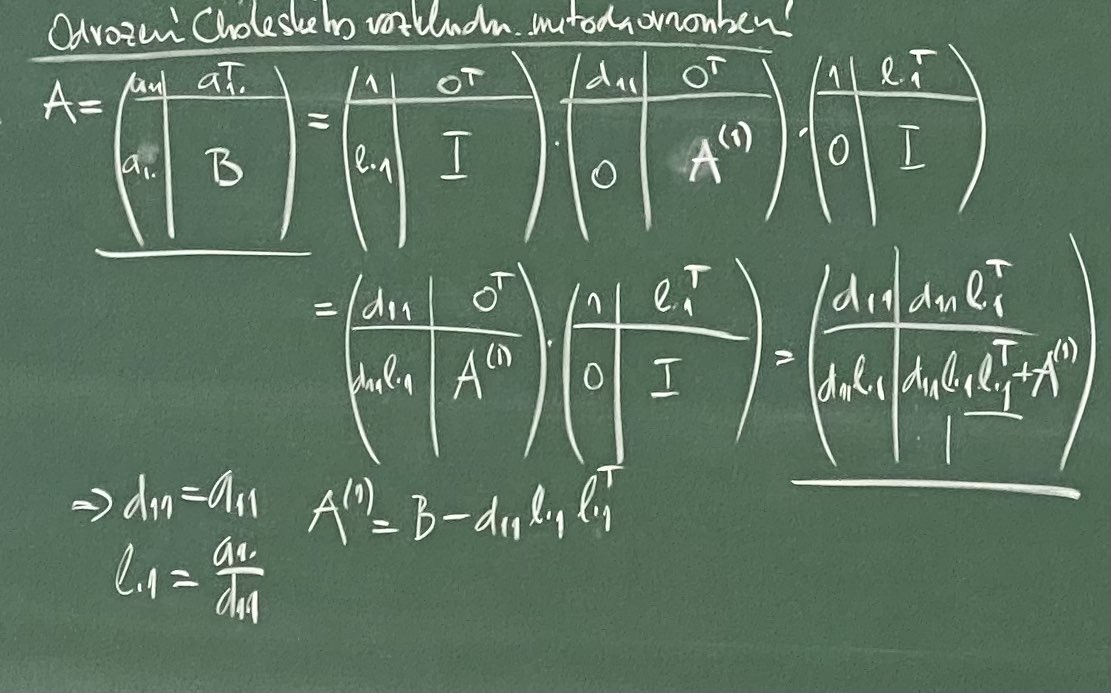
\includegraphics[width=0.9\linewidth]{images/12-10-odvozeni.jpg}
\end{center}




\subsection{Submaticová metoda}
Right looking approach (k,i,j varianta)

\begin{minipage}{0.95\linewidth}
\begin{verbatim}
for k  = 1 ... n 
    d_{kk} = a_{kk}
    for i = k+1 ... n
        l_{ik}  = a_{ik}/d_{kk}
    end
    for i = k+1 ... n
        for j = k+1 ... n
            a_{ij} = a_{ij} - l_{ik} a_{kj}
        end j
    end i
end k
\end{verbatim}
\end{minipage}


\subsection{Sloupcová metoda}
Left looking approach (j,k,i varianta)

\begin{minipage}{0.95\linewidth}
\begin{verbatim}
for j = 1 ... n 
    for k = 1 ... j-1
        for i = k+1 ... n
            a_{ij} = a_{ij} - l_{ik}a_{kj}
        end i
    end k
    d_{jj} = a_{jj}
    for i = j+1 ... n
        l_{ij} = a_{ij} / d_{jj}
    end i 
end j
\end{verbatim}    
\end{minipage}


\begin{remark}
    Obě metody lze vylepšit, stačí provádět cykly pouze přes nenulové prvky
\end{remark}

\begin{remark}
    Pro hustou matici lze výpočet provádět přímo v matici \matA 
\end{remark}



\begin{example}
    
    
\begin{center}
    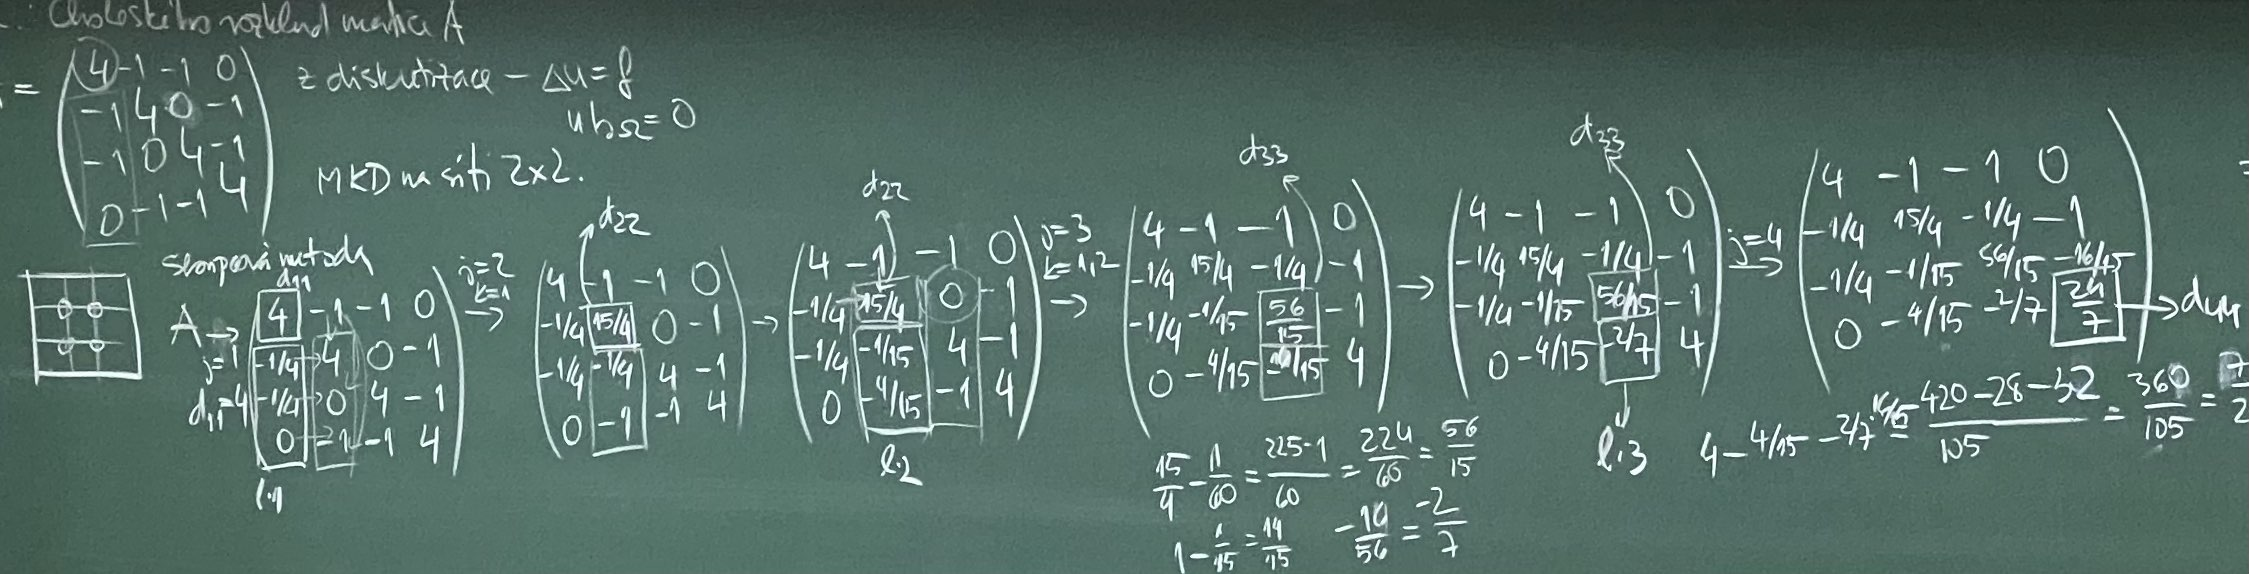
\includegraphics[width=\linewidth]{images/12-10-example.jpg}
\end{center}

Z toho dostáváme 
\begin{equation*}
    \mathbb{L} = \begin{pmatrix}
        1 & 0 & 0 & 0 \\
        -\frac{1}{4} & 1 & 0 & 0 \\
        -\frac{1}{4} & -\frac{1}{15} & 1 & 0 \\
        0 & -\frac{4}{15} & -\frac{2}{7} & 1 
        \end{pmatrix} , \mathbb{D} = \begin{pmatrix}
            4 & 0 & 0 & 0 \\
            0 & \frac{15}{4} & 0 & 0 \\
            0 & 0 & \frac{56}{15} & 0 \\
            0 & 0 & 0 & \frac{24}{7} 
            \end{pmatrix}
\end{equation*}
a platí $\mathbb{L}\mathbb{D}\mathbb{L}^T = \mathbb{A}$.\\
Pro řešení $\mathbb{A}x = b$ řešíme $\mathbb{L}y = b, \mathbb{D}z = y, \mathbb{L}^T x = z$
\end{example}

\begin{remark}

    $l_{32} \neq 0$ ačkoliv $a_{32} = 0$, na pozici 3,2 došlo k zaplnění.

    Faktor $\mathbb{L}$ má obecně více nenulových prvků než \matA : \matA je řídká $\centernot\implies$ $\mathbb{L}$ je řídká, $\mathbb{L}$ ,může být i kompletně zaplněná.\\
    Datové struktury neumožňují snadno přidat nový nenulový prvek, dynamické datové struktury jsou drahé
    $\implies$ je třeba umět předpovědět množství a polohy nenulových prvků, tj. určit strukturu 
    $\mathbb{L}$ na základě struktury \matA .
\end{remark}


\subsection{Popis struktury řídkých matic}
Matici $\mathbb{A}\in\mathbb{R}^{n,n}$ přiřadíme graf $G(\mathbb{A}) = (V,E)$, $V=\hat{n}$.\\
\begin{equation*}
    E\subset V\times V \dots (i,j)\in E \Leftrightarrow a_{ij} \neq 0 
\end{equation*}
Pro strukturně nesymetrické matice je $G(\mathbb{A})$ orientovaný.

\begin{center}
    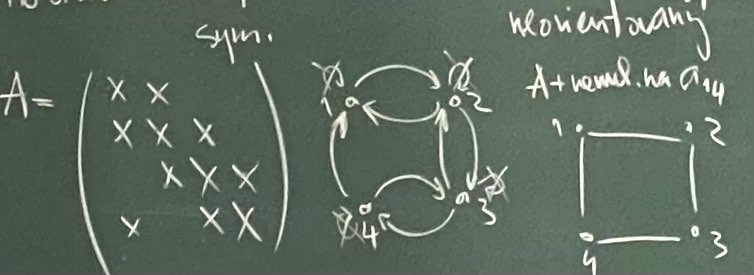
\includegraphics[width=0.5\linewidth]{images/12-10-definice-pridruzeneho-grafu.jpg}
\end{center}

\begin{remark}
    Grafy matic pocházející z diskretizací PDR (MKD, MKO, MKP) často jsou totožné s grafem sítě. 
\end{remark}


\subsection{Vznik zaplnění}
Nechť \matA je SPD
\begin{center}
    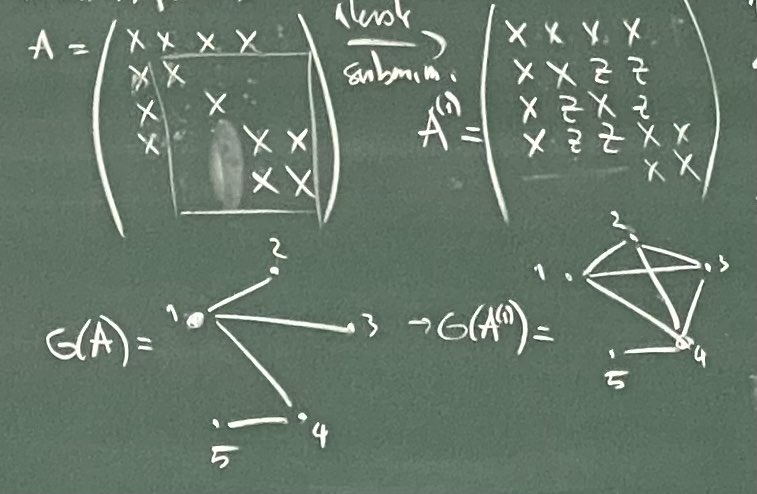
\includegraphics[width=0.5\linewidth]{images/12-10-matice-s-pridruzenym-grafem.jpg}
\end{center}

1 sloupec "otiskne" svoji strukturu do všech sloupců j, pro které $a_{1j}\neq0$.\\
Po provedení 1 kroku submaticového algoritmu se incidentní vrcholy pivota propojí do kliky (každý s každým), tedy vzniká zaplnění.


\end{document}